\subsection{Kademlia}
Nato nel 2002, questo protocolo si basa su DSM, utilizza delle tabelle di hash distrinuite dove ogni risorsa pubblicata viene associata ad una chiave.

\subsubsection{Distanza tra identificatori}
Kademlia usa una chiave di 160 bit per gli identificatori, nella fase di pubblicazione, la coppia chiave valore viene associata alla risorsa sulla base del id del nodo più vicino alla risorsa.
La distanza si ottiene facendo un XOR logico.
\subsubsection{Struttura dati dei nodi}
Ogni nodo ha 160 k-buckets, un bucket è una lista di massimo k tuple (indirizzi IP, UDP port, Node ID) correlate a nodi che hanno una distanza dal nodo attaule compresa tra $2^i$ e $2^{i+1}$ con i tra 0 e 159.


\begin{figure}[h!]
    \centering
    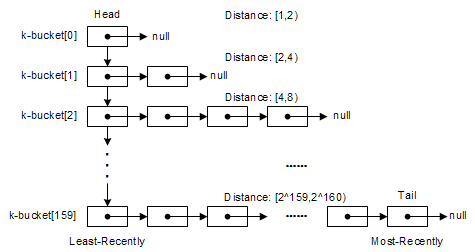
\includegraphics[width=0.5\linewidth]{imgs/12 - kbuckets.png}
    \label{fig:k-buckets}
    \caption{Esempio di struttura dei k-buckets}
\end{figure}

Quando un nodo riceve un messaggio da un'altro nodo, controlla la k-bucket che contiene la descrizione del sender, se questa descrizione è presente, il nodo muove la richiesta in coda a tutte le richieste, se la descrizione del pacchetto è assente, il noda scarta.

\subsubsection{Protocolllo RPCs}
kademlia ha 4 RPCs:

\begin{itemize}
    \item PING: il peer è online
    \item STORE: salva un dato 
    \item FIND NODE
    \item FIND VALUE
\end{itemize}

\subsubsection{Ricerca di nodi recursiva}

\begin{figure}[h!]
    \centering
    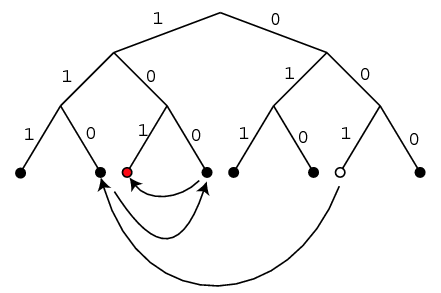
\includegraphics[width=0.5\linewidth]{imgs/13 - kademlia tree.png}
    \label{fig:kademlia-tree}
    \caption{Illustrazione del lookup dei nodi}
\end{figure}

Per publicare una risorsa (coppia chiave valore), il nodo n cerca per i k nodi vicini e invoca il metodo STORE.

Per effettuare il lookup(ricerca) della risorsa, il nodo chiama il motodo FIND VALUE di una certa chiave e propaga a tutti i nodi adiaceni, ripetere finchè non si ottiene il valore della chiave.
